\documentclass[conference]{IEEEtran}
\IEEEoverridecommandlockouts
% The preceding line is only needed to identify funding in the first footnote. If that is unneeded, please comment it out.
%Template version as of 6/27/2024

\usepackage{cite}
\usepackage{amsmath,amssymb,amsfonts}
%\usepackage{algorithmic}
\usepackage{algorithm}
\usepackage{algpseudocode}
\usepackage{verbatim}
\usepackage[dvipdfmx]{graphicx}
\usepackage{textcomp}
\usepackage{xcolor}
\def\BibTeX{{\rm B\kern-.05em{\sc i\kern-.025em b}\kern-.08em
    T\kern-.1667em\lower.7ex\hbox{E}\kern-.125emX}}
\begin{document}

\title{Motion Comparison for Dance Skill Improvement \\via Sequential Unsupervised Segmentation}

\author{
\IEEEauthorblockN{
Ken Kajiwara\IEEEauthorrefmark{1},
Issei Saito\IEEEauthorrefmark{1}, 
Tomoaki Nakamura\IEEEauthorrefmark{1},
Daichi Mochihashi\IEEEauthorrefmark{2},
and Koki Mimura\IEEEauthorrefmark{3}
}
\IEEEauthorblockA{\IEEEauthorrefmark{1}The University of Electro-Communications, Tokyo, Japan \\
}
\IEEEauthorblockA{\IEEEauthorrefmark{2}The Institute of Statistical Mathematics, Tokyo, Japan}
\IEEEauthorblockA{\IEEEauthorrefmark{3}National Center of Neurology and Psychiatry, Tokyo, Japan}
E-mail: k2532028@edu.cc.uec.ac.jp}

\def\bq{\begin{equation}}
\def\eq{\end{equation}}
\def\beq{\begin{eqnarray}}
\def\eeq{\end{eqnarray}}
\def\ba{\begin{array}}
\def\ea{\end{array}}
\def\bc{\begin{center}}
\def\ec{\end{center}}

\def\dsum{\sum\limits}
\def\disp{\displaystyle}
\def\ejw{e^{j\omega}}
\def\ejwi{e^{j\omega_{i}}}
\def\e-jwi{e^{-j\omega_{i}}}
\def\dfrac#1#2{\disp{\frac{#1}{#2}}}
\def\teigi{\stackrel{\triangle}{=}}


%\def\b0{\mbox{\boldmath$0$}}


\if0
\def\baa{\mbox{\boldmath$a$}}
\def\bb{\mbox{\boldmath$b$}}
\def\bcc{\mbox{\boldmath$c$}}
\def\bd{\mbox{\boldmath$d$}}
\def\be{\mbox{\boldmath$e$}}
\def\bff{\mbox{\boldmath$f$}}
\def\bg{\mbox{\boldmath$g$}}
\def\bh{\mbox{\boldmath$h$}}
\def\bi{\mbox{\boldmath$i$}}
\def\bj{\mbox{\boldmath$j$}}
\def\bk{\mbox{\boldmath$k$}}
\def\bl{\mbox{\boldmath$l$}}
\def\bm{\mbox{\boldmath$m$}}
\def\bn{\mbox{\boldmath$n$}}
\def\bo{\mbox{\boldmath$o$}}
\def\bp{\mbox{\boldmath$p$}}
\def\bqq{\mbox{\boldmath$q$}}
\def\br{\mbox{\boldmath$r$}}
\def\bs{\mbox{\boldmath$s$}}
\def\bt{\mbox{\boldmath$t$}}
\def\bu{\mbox{\boldmath$u$}}
\def\bv{\mbox{\boldmath$v$}}
\def\bw{\mbox{\boldmath$w$}}
\def\bx{\mbox{\boldmath$x$}}
\def\by{\mbox{\boldmath$y$}}
\def\bz{\mbox{\boldmath$z$}}

\def\bA{\mbox{\boldmath$A$}}
\def\bB{\mbox{\boldmath$B$}}
\def\bC{\mbox{\boldmath$C$}}
\def\bD{\mbox{\boldmath$D$}}
\def\bE{\mbox{\boldmath$E$}}
\def\bF{\mbox{\boldmath$F$}}
\def\bG{\mbox{\boldmath$G$}}
\def\bH{\mbox{\boldmath$H$}}
\def\bI{\mbox{\boldmath$I$}}
\def\bJ{\mbox{\boldmath$J$}}
\def\bK{\mbox{\boldmath$K$}}
\def\bL{\mbox{\boldmath$L$}}
\def\bM{\mbox{\boldmath$M$}}
\def\bN{\mbox{\boldmath$N$}}
\def\bO{\mbox{\boldmath$O$}}
\def\bP{\mbox{\boldmath$P$}}
\def\bQ{\mbox{\boldmath$Q$}}
\def\bR{\mbox{\boldmath$R$}}
\def\bS{\mbox{\boldmath$S$}}
\def\bT{\mbox{\boldmath$T$}}
\def\bU{\mbox{\boldmath$U$}}
\def\bV{\mbox{\boldmath$V$}}
\def\bW{\mbox{\boldmath$W$}}
\def\bX{\mbox{\boldmath$X$}}
\def\bY{\mbox{\boldmath$Y$}}
\def\bZ{\mbox{\boldmath$Z$}}
\fi



\if0
\def\b0{\bf{0}}
\def\bPhi{\mbox{\boldmath$\Phi$}}
\def\bomega{\mbox{\boldmath$\omega$}}
\def\bLambda{\mbox{\boldmath$\Lambda$}}
\def\blambda{\mbox{\boldmath$\lambda$}}
\def\bmu{\mbox{\boldmath$\mu$}}
\def\bnu{\mbox{\boldmath$\nu$}}
\def\bSigma{\mbox{\boldmath$\Sigma$}}
\def\bPhi{\mbox{\boldmath$\Phi$}}
\def\balpha{\mbox{\boldmath$\alpha$}}
\def\bTheta{\mbox{\boldmath$\Theta$}}
\def\btheta{\mbox{\boldmath$\theta$}}
\def\bGamma{\mbox{\boldmath$\Gamma$}}
\def\bPsi{\mbox{\boldmath$\Psi$}}
\def\bDelta{\mbox{\boldmath$\Delta$}}
\def\bPi{\mbox{\boldmath$\Pi$}}
\fi

\makeatletter
\def\lddots{\mathinner{\mkern1mu\raise\p@\vbox{\kern7\p@\hbox{.}}\mkern2mu
\raise4\p@\hbox{.}\mkern2mu\raise7\p@\hbox{.}\mkern1mu}}
\makeatother


\def\argmax{\mathop{\rm argmax}}




\def\baa{{ \boldsymbol a}}
\def\bb{{ \boldsymbol b}}
\def\bcc{{ \boldsymbol c}}
\def\bd{{ \boldsymbol d}}
\def\be{{ \boldsymbol e}}
\def\boldsymbolf{{ \boldsymbol f}}
\def\bg{{ \boldsymbol g}}
\def\bh{{ \boldsymbol h}}
\def\bi{{ \boldsymbol i}}
\def\bj{{ \boldsymbol j}}
\def\bk{{ \boldsymbol k}}
\def\bl{{ \boldsymbol l}}
\def\bm{{ \boldsymbol m}}
\def\bn{{ \boldsymbol n}}
\def\bo{{ \boldsymbol o}}
\def\bp{{ \boldsymbol p}}
\def\bqq{{ \boldsymbol q}}
\def\br{{ \boldsymbol r}}
\def\bs{{ \boldsymbol s}}
\def\bt{{ \boldsymbol t}}
\def\bu{{ \boldsymbol u}}
\def\bv{{ \boldsymbol v}}
\def\bw{{ \boldsymbol w}}
\def\bx{{ \boldsymbol x}}
\def\by{{ \boldsymbol y}}
\def\bz{{ \boldsymbol z}}

\def\bA{{ \boldsymbol A}}
\def\bB{{ \boldsymbol B}}
\def\bC{{ \boldsymbol C}}
\def\bD{{ \boldsymbol D}}
\def\bE{{ \boldsymbol E}}
\def\bF{{ \boldsymbol F}}
\def\bG{{ \boldsymbol G}}
\def\bH{{ \boldsymbol H}}
\def\bI{{ \boldsymbol I}}
\def\bJ{{ \boldsymbol J}}
\def\bK{{ \boldsymbol K}}
\def\bL{{ \boldsymbol L}}
\def\bM{{ \boldsymbol M}}
\def\bN{{ \boldsymbol N}}
\def\bO{{ \boldsymbol O}}
\def\bP{{ \boldsymbol P}}
\def\bQ{{ \boldsymbol Q}}
\def\bR{{ \boldsymbol R}}
\def\bS{{ \boldsymbol S}}
\def\bT{{ \boldsymbol T}}
\def\bU{{ \boldsymbol U}}
\def\bV{{ \boldsymbol V}}
\def\bW{{ \boldsymbol W}}
\def\bX{{ \boldsymbol X}}
\def\bY{{ \boldsymbol Y}}
\def\bZ{{ \boldsymbol Z}}


\def\b0{{\boldsymbol 0}}
\def\bPhi{{\boldsymbol\Phi}}
\def\bomega{{\boldsymbol\omega}}
\def\bLambda{{\boldsymbol\Lambda}}
\def\blambda{{\boldsymbol\lambda}}
\def\bmu{{\boldsymbol\mu}}
\def\bsigma{{\boldsymbol\sigma}}
\def\bnu{{\boldsymbol\nu}}
\def\bepsilon{{\boldsymbol\epsilon}}
\def\bphi{{\boldsymbol\phi}}
\def\bSigma{{\boldsymbol\Sigma}}
\def\bPhi{{\boldsymbol\Phi}}
\def\balpha{{\boldsymbol\alpha}}
\def\bTheta{{\boldsymbol\Theta}}
\def\btheta{{\boldsymbol\theta}}
\def\bGamma{{\boldsymbol\Gamma}}
\def\bPsi{{\boldsymbol\Psi}}
\def\bDelta{{\boldsymbol\Delta}}
\def\bPi{{\boldsymbol\Pi}}
\def\bXi{{\boldsymbol\Xi}}
\def\bxi{{\boldsymbol\xi}}
\def\bomega{{\boldsymbol\omega}}
\def\bOmega{{\boldsymbol\Omega}}

\def\balpha{{\boldsymbol\alpha}}
\def\bbeta{{\boldsymbol\beta}}
\maketitle

\begin{abstract}
本研究の目的は,ダンスやスポーツなど熟練度の異なる複数人の連続動作の違いを,単位動作毎に
定量的・視覚的に比較可能な支援システムを構築することである.
そのためには,複数人の連続動作から共通する単位動作を抽出し,単位動作毎に各個人の動作の違いを解析する必要がある.
このような連続動作から単位動作を自動的に抽出する技術は分節化と呼ばれており,そのような分節化が可能な手法の一つに
Gaussian Process Hidden Semi-Markov Model(GP-HSMM)がある.GP-HSMMは,高い表現力を持つ一方で,学習に多くの時間を要するため,
高次元·長時間のデータを解析することが難しいという課題があった.また,単位動作がノンパラメトリックな確率モデルであるガウス過程で表現されているため,
個人間の動作の違いを定量化することができないという問題もある.そこで.本研究では,これら課題に対処するために,ガウス過程のカーネル関数を近似する基底関数をRandom Fourier Features(RFF)
によって導出し,単位動作を導出した基底関数を利用した線形回帰モデルで表現する.これによりガウス過程の計算がよりシンプルな線形回帰モデルに
なるため計算を効率化することができる.
さらに,逐次学習を導入することで,初期モデルで学習した熟練者の動作で学習したモデルに対して,新たな被験者の動作を
逐次的に学習することができる.線形回帰モデルでは,単位動作が低次元のパラメータで表現されているため,追加学習前後のパラメータを定量的に比較することで,
熟練者と新たな被験者の単位動作の違いを定量的に比較することが可能となる.評価実験では,体操およびダンスの
公開モーションキャプチャデータセットを用いて,提案手法が従来手法と同等の分節化精度を維持しながら,
従来の手法ではおよそ87時間かかった処理がおよそ3分に大幅に短縮でき,複数被験者の動作の違いを関節単位で可視化・定量化できる支援システムとして有効であることを示した.
\end{abstract}

\begin{IEEEkeywords}
computational efficiency, Gaussian process, motion analysis, random Fourier features, time-series modeling, unsupervised segmentation, sequential learning, motion comparison, Dance skill improvement, MCMC optimization.
\end{IEEEkeywords}

\section{Introduction}
近年,モーションキャプチャ技術の発展により,人間の複雑な動作を高精度かつ連続的に記録・解析することが可能になってきた\cite{Balazia2018, 3DPW2018, Thoker2021, Lam2023, Suo2024, DanceMVP2024}.
ダンスやスポーツなどの領域では,従来,動作指導が指導者の主観的な経験や感覚に基づいて行われてきたが,動作を定量的に評価する手法の需要が高まっている.

Gaussian Process Hidden Semi-Markov Mode(GP-HSMM)\cite{Nakamura2017}は,動作の時系列データを意味のある単位に自動的に分割し,
各セグメントをガウス過程により柔軟にモデル化できる点で有効なアプローチである.特に,動作の分節化と分析を一貫して処理できる点が有用である.
しかしながら,GP-HSMMはその柔軟性と引き換えに,ガウス過程の計算コストが高く,データ規模が増えるにつれて実用的な応用が困難になるという問題を抱えている.

この問題に対処するため,Random Fourier Features(RFF)\cite{Rahimi2007} によりガウス過程のカーネル関数を近似する基底関数を導出し,
導出した基底関数を用いて単位動作を線形回帰モデルで表現することで,計算負荷を大幅に削減することを可能にし,動作解析の可能性が広がった.
本研究では,Random Fourier Features(RFF)\cite{Rahimi2007} によってサンプリングされる周波数ベクトルと位相パラメータを Metropolis-Hastings 法に
基づくマルコフ連鎖モンテカルロ(MCMC)\cite{Hastings1970} で最適化し,近似精度を統計的に安定化させている.

また,従来のGP-HSMMは,観測点の増加に応じて潜在状態集合と各状態のガウス過程共分散行列が高次元化する非パラメトリック・ベイズモデルであるため,厳密なベイズ推論にはすべての観測データを一括で学習する必要があり,
新たな被験者の動作を柔軟に取り入れることが難しく,複数被験者間の動作比較も困難であった.そこで本研究では,逐次学習\cite{Broderick2013}を導入する.これにより,初期データで得た知見を活かしつつ,新たな被験者の動作を段階的に学習することで,熟練度の違う被験者の動作の特徴を,各動作セグメントに基づいて定量的に比較・評価することが可能となる.

体操およびダンスの公開モーションキャプチャデータセットを用いた評価実験により,提案手法の有効性を検証した.
体操データセットにおいては,RFF-GP-HSMMにMetropolis-Hastings 法を用いた MCMC(Markov Chain Monte Carlo)法\cite{Hastings1970}を導入し,
RFFで使用される周波数ベクトルおよび位相パラメータを最適化して近似精度を安定化させ,
正解ラベルとの正規化ハミング距離の平均値および標準偏差が,MCMCを導入していないRFF-GP-HSMMよりも改善され,提案手法がGP-HSMMと同等の分節精度であることを示した.
また,288万点のデータを含むダンスデータセットに対しては,従来のGP-HSMMでは解析におよそ87時間を要したのに対し,提案手法ではおよそ3分で解析が完了し,実用的な処理時間で解析可能となった.
さらに,逐次学習の導入により,熟練度の異なる2名のダンサーの動作を振り付け単位で定量的に比較・評価することが可能となり,改善すべき関節動作を可視化する比較支援システムを構築した.

本研究では,Random Fourier Features(RFF)\cite{Rahimi2007} によりガウス過程カーネルを近似し,単位動作を線形回帰モデルで
表現して計算負荷を大幅に削減するとともに,逐次学習\cite{Broderick2013} を導入して熟練度の異なる複数人の連続動作の違いを,単位動作毎に
定量的・視覚的に比較・評価できる新たなフレームワークを提案する.
本手法は,従来法では困難であった動作データへの適用と個人差に
基づく動作解析の両立を可能にし,実用性と拡張性を兼ね備えた動作理解のアプローチを示すものである.

\section{Related work}
近年,モーションキャプチャ技術の進展により,人間の動作を高精度に解析する研究が活発に行われている\cite{Balazia2018, 3DPW2018, Thoker2021, Lam2023, Suo2024, DanceMVP2024}.
たとえば、BalaziaとSojka\cite{Balazia2018}は,CMU MoCapデータベースを用いて,31関節から得られる3D時系列データに対し,
LDAとMaximum Margin Criterion(MMC)を組み合わせた特徴抽出を行い,歩行者識別において従来手法を上回る精度を
達成した.これは、モーションキャプチャを用いた単純な動作の識別に関する有効な手法の一例である.

また,ダンスのような複雑な動作を対象とした研究も進展している.
DanceMVP\cite{DanceMVP2024}では,69,300秒に及ぶダンス動作と音楽を含むデータセット
ImperialDanceを開発し,5つのジャンル,20曲の音楽,20種類の振り付けから構成される大規模マルチモーダルデータを収録している.
このデータセットは,語彙認識,パフォーマンススコアリング,リズム整合性評価といった複数タスクを統合的に扱う自己教師あり学習フレームワーク
のために設計されており,異なる熟練度のダンサーによる繰り返し動作を通じて,技能の違いを捉えるためのものとなっている.

しかしながら,この研究では,動作全体をスコアリングや分類することに主眼が置かれており,分類においては専門家による
手動のアノテーション作業が必要不可欠であるため,一般のユーザーや現場レベルで広く受け入れられるような動作解析手法としては不十分
である.そのため,一般的に受け入れやすく,かつ自動的に処理可能な解析手法として,振り付けなどの個々の動作単位ごとに
習熟度の違いを定量的に分析可能な効率的手法の開発が求められている.

この課題に対して,教師なし分割\cite{Fox2011, Matsubara2014, Sener2018, Bojanowski2014, Huang2016, Richard2017}は有望なアプローチとして注目されており,繰り返し現れるパターンを自動的に抽出し,
複雑な時系列データの構造解析を可能にする.産業応用を含む様々な実世界のタスクにおいて重要な役割を果たす一方,従来の手法では,
セグメントの開始・終了点とカテゴリを同時に推定する必要があるため,組み合わせ爆発による計算コストが問題となり,
その回避のために導入されたヒューリスティックな仮定は,タスク依存性が高いという課題を抱えている.

このような背景のもと本研究では,この課題に対処するためにGaussian Process Hidden Semi-Markov Model(GP-HSMM)\cite{Nakamura2017}に着目する.
このモデルは,ガウス過程を非パラメトリックモデルとして用いて,繰り返し現れる複雑なパターンを捉え,HSMM(隠れセミマルコフモデル)
によってそれらのパターンの持続時間をモデル化する.確率的生成モデルに基づくこの手法は,従来手法よりも複雑な時系列データの高精度な
セグメンテーションを可能にし,かつ高い解釈性を有する.実際に,GP-HSMMはその解釈性とセグメンテーション精度のバランスの良さから,
多くの研究で活用されている.たとえば,MimuraらはGP-HSMMに階層的ディリクレ過程を組み込むことで,マーモセットの特徴的な行動を
教師なしで抽出できることを示した\cite{Mimura2024}.また,製造現場では作業者の行動解析に応用され,作業パターンだけでなく,オペレーターごとの
特性や熟練度の違いも明らかにされている\cite{Saito2023a}.ロボット学習の分野においては,連続的なタスクを原始的な動作に分割する目的で本手法が
利用されている\cite{Mo2023}.

高精度な教師なしセグメンテーション手法として有効である一方で,GP-HSMMはガウス過程に起因する計算負荷の高さという問題を抱えている.

この課題に対する有望な解決策として,カーネルをRandom Fourier Features(RFF)によって近似する基底関数
の導出がある\cite{Rahimi2007}.RFFは,スケーラブルなGPLVM(Gaussian Process Latent Variable Model)\cite{Zhang2023}\cite{Li2024}を可能にし,精度を
損なうことなくハイブリッドHMMの高速化を実現してきた\cite{Jung2020}.これらの結果に動機づけられ,我々はGP-HSMMにRFFを導入した.
ただし,RFFは近似手法であるため,性能が不安定であるという問題がある.

そこでさらに,本研究ではMetropolis-Hastings 法を用いた MCMC(Markov Chain Monte Carlo)法\cite{Hastings1970}を導入し,
RFFで使用される周波数ベクトルおよび位相パラメータを最適化することで,近似のばらつきを抑え,
より安定した性能を実現した.

加えて,ベイズ線形回帰における事後分布の逐次更新則に基づき,逐次学習\cite{Broderick2013}導入することで,一度学習した熟練者モデルを保持したまま,
新たな中級者のデータを段階的に統合し,複数人の動作比較・評価を効率的に行うことが可能となった.

\section{Method}

\subsection{Generative process}\label{AA}
Fig.~\ref{fig:model} に提案する RFF-GP-HSMM のグラフィカルモデルを示す.  
本モデルでは,時系列データ $\bS$ が次の生成過程を経て得られると仮定する.

\begin{figure}[t]
  \begin{center}
    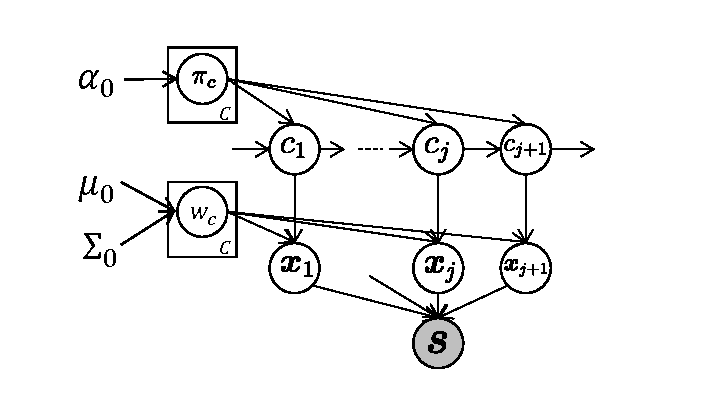
\includegraphics[scale=0.6]{fig/model.pdf}
    \caption{RFF-GP-HSMM のグラフィカルモデル.}
    \label{fig:model}
  \end{center}
  \vspace{-0.4cm}
\end{figure}

まず,遷移確率 $\pi_c$ をディリクレ分布(パラメータ $\alpha_0$)から生成する.
%
\begin{eqnarray}
\pi_c &\sim& P(\pi \mid \alpha_0).
\end{eqnarray}
%
次に,第 $j$ セグメントのクラス $c_j$ を,直前のクラス $c_{j-1}$ と遷移確率 $\pi_c$ に基づいて生成する.
%
\begin{eqnarray}
c_j &\sim& P(c \mid c_{j-1}, \pi_c).
\end{eqnarray}
%

従来の GP-HSMM では,各セグメント $\bx_j$ はガウス過程によって生成されると仮定する.  
一方,RFF-GP-HSMM では,各セグメントを線形回帰で生成する.  
回帰重み $\bw_c$ は平均 $\bmu_0$,共分散行列 $\bSigma_0$ のガウス分布から生成する.
%
\begin{eqnarray}
\bw_c &\sim& \mathcal{N}(\bw \mid \bmu_0, \bSigma_0).
\end{eqnarray}
%
クラス $c_j$ に対応するセグメント $\bx_j$ は,重み $\bw_{c_j}$ を用いた線形回帰によって生成される.
%
\begin{eqnarray}
\bx_j &\sim& p(\bx \mid \bw_{c_j}).
\end{eqnarray}

観測された時系列データ $\bS$ は,これらのセグメント $\bx_j$ を連結することで得られる.  
ただし,単純な線形回帰だけでは複雑な時系列パターンを十分に捉えられない.  
そこで RFF-GP-HSMM では,Random Fourier Features (RFF) により導出される基底関数を用いた線形回帰\cite{Rahimi2007} を採用し,モデル表現力を高めている.

\subsection{Gaussian Processes}
GP-HSMMでは,各クラスの時刻$t'$の出力値$x'$の予測にガウス過程を用いることで複雑に変化する時系列データを表現している.
ガウス過程は,$\bphi$を基底関数とした線形回帰モデル$x' = \bw^T \bphi(t')$に対して,重み$\bw$の周辺化とカーネルトリックを適用した確率モデルである.
%%
%\begin{equation}
%p(x'|t',\bX_c, \bt)  = \int {\mathcal N}(x'| \bw^T \phi(t'), \beta^{-1})  p(\bw| \bX_c, \bt) d \bw \label{eq:lin_reg}
%\end{equation}
%%
ガウス過程では,クラス$c$に分類された分節の集合$\bX_c$と,対応するタイムステップの集合$\bt_c$が与えられたとき,時刻$t'$の出力$x'$の予測分布は次式のガウス分布となる.
%
\begin{equation}
p(x'|t',\bX_c, \bt_c)  = {\mathcal N}(\bk^{T}\bK^{-1}\bX_c, k(\hat{t'}, \hat{t'})-\bk^{T}\bK^{-1}\bk), \label{eq:gp_pred}
\end{equation}
%
$k(\cdot, \cdot)$はカーネル関数であり,$\bK$は$q$行$p$列の要素が次式となる行列である.
%
\begin{equation}
\label{equ:covariance_func}
K(p, q)=k(t_{p},t_{q})+\beta^{-1}\delta_{pq}, 
\end{equation}
%
$t_p$と$t_q$はそれぞれ,$\bt_c$の$p$番目の要素と$q$番目の要素であり,$\beta$と$\delta_{pq}$はそれぞれノイズ成分を表すパラメータとデルタ関数である.
$\bk$は,$p$番目の要素が$k(t_p, t')$となるベクトルである.
本稿では,カーネル関数として次式のRBFカーネルを用いる.
%
\begin{equation}
k(t_p,t_q)=\exp(-\frac{1}{2}||t_{p}-t_{q}||^{2}), \label{eq:rbf}
\end{equation}
%
カーネルを用いることで,基底関数$\bphi(\cdot)$を直接計算せずに,その内積である$k(t_p,t_q)=\bphi(t_p)^T \bphi(t_q)$を計算することで,非線形高次元空間で柔軟に入出力の関係を捉えることができる.

GP-HSMMでは,出力が多次元ベクトル$\bx'$の場合は,各次元が独立に生成されると仮定し,その生成確率を次式のように計算する.
%
\begin{equation}
\label{equ:multi_dim}
{\mathcal GP(\bx'|t', \bX_{c}, \bt)} = \prod_d^D p(\bx'^{(d)}|t', \bX^{(d)}_{c}).
\end{equation}
%
ただし,上付きの添字$d$は,それぞれの変数の$d$次元目を表している.

ガウス過程では,式(\ref{eq:gp_pred})の計算に,$\bK$の逆行列演算を含んいる.
$\bX_c$に含まれるデータ点数を$N_c$とすると,$\bK$のサイズは$N_c \times N_c$となる.
すなわち,処理する時系列データ点の数$N_c$が多くなれば行列$\bK$のサイズも大きくなり,その逆行列の演算に多くの計算時間が必要になる.
これが現状のGP-HSMMの計算時間のボトルネックとなっている.

\subsection{Gaussian process approximation using RFF}
ガウス過程では,カーネルトリックにより,基底関数$\bphi$を直接計算することなく非線形高次元空間で入出力の対応関係を捉えている.
一方で,もし$k(t_p,t_q)\approx \bphi(t_p)^T \bphi(t_q)$となる,内積をとるとRBFカーネルの近似になるような基底関数$\bphi$を導出できれば,$\bK$を計算する必要のない線形回帰モデル$x'=\bw^T \bphi(t')$を適用することができる.
このような,カーネルからそのカーネルを近似可能な基底関数を求める方法がRandom Fourier Feature (RFF)\cite{Rahimi2007}である.

RFFでは,まずカーネル関数のフーリエ変換を考える.
式(\ref{eq:rbf})のRBFカーネルを$\Delta = t_p - t_q$を入力とする関数$k'(\Delta)=\exp( -||\Delta||^2/2 )$とし,$k'(\Delta)$をフーリエ変換すると次式のガウス分布となる.
%
\begin{equation}
p(\omega) = (2 \pi)^{-\frac{D}{2}} \exp(-\frac{1}{2}||w||^2)
\end{equation}
%
次に,この$p(\omega)$をフーリエ逆変換し,もとのカーネル関数を復元する.
%
\begin{eqnarray}
k(t_p,t_q) &=& k'(\Delta) \\
&=& \int_\mathbb{R} p(\omega) \exp( i \omega (t_p - t_q) ) d \omega \\
&=& \int_\mathbb{R} p(\omega)\cos(\omega (t_p - t_q)) + i \sin(\omega (t_p - t_q)) d \omega \nonumber \\
\end{eqnarray}
%
この式変形にはオイラーの公式$\exp(iz) = \cos(z) + i \sin(z)$を用いた.
さらに,カーネル関数の出力値は実数となるため
%
\begin{eqnarray}
k(t_p,t_q) = \int_\mathbb{R} p(\omega)\cos(\omega (t_p - t_q)) d \omega 
\end{eqnarray}
%
となる.次に,$b \sim {\rm Uniform}(0, 2 \pi)$となる乱数($p(b) = \frac{1}{2 \pi}$)を導入し,$b$での周辺化を考えると
%
\begin{eqnarray}
&&\int_0^{2 \pi} p(b) p(\omega)\cos(\omega (t_p - t_q)) d b = p(\omega)\cos(\omega (t_p - t_q)) \nonumber \\ \\
&&\int_0^{2 \pi} p(b) p(\omega)\cos(\omega (t_p + t_q) + 2 b) d b \\
&&~~~~~~~~~= \left[ \frac{1}{4 \pi} p(\omega)\sin(\omega (t_p + t_q) + 2 b)  \right]_0^{2 \pi}=0 
\end{eqnarray}
%
が成り立つため,$k(t_p,t_q)$は次式のように変形することができる.
%
\begin{eqnarray}
k(t_p,t_q) = \int_\mathbb{R} \int_0^{2 \pi} p(b) p(\omega) \left\{ \cos(\omega (t_p + t_q) + 2 b) \right. \nonumber \\
~~~ \left. +\cos(\omega (t_p - t_q)) \right\} db d \omega 
\end{eqnarray}
%
ここで,$A=\omega t_p +b, B = \omega t_q +b $とすると,
%
\begin{eqnarray}
\cos(A+B) + \cos(A-B)= 2 \cos(A)\cos(B)
\end{eqnarray}
%
となり,次式のように変形することができる.
%
\begin{eqnarray}
k(t_p,t_q) &=& \int_\mathbb{R} \int_0^{2 \pi} p(b) p(\omega) \sqrt{2} \cos(\omega t_p +b) \nonumber \\
&&~~~~~~ \times \sqrt{2} \cos(\omega t_q +b) db d \omega 
\end{eqnarray}
%
この積分を$M$個のサンプル$\omega^{(m)}, b^{(m)}$でモンテカルロ近似する.
%
\begin{eqnarray}
\omega^{(m)} &\sim& p(\omega), \\
b^{(m)} &\sim& {\rm Uniform}(0, 2 \pi), \\
{k}(t_p,t_q) &=& \frac{1}{M} \sum_m  \sqrt{2}\cos(\omega^{(m)} t_p +b^{(m)}) \nonumber \\
&&~~~~~~~~ \times \sqrt{2}\cos(\omega^{(m)} t_q +b^{(m)})  \label{eq:rff_mc}
\end{eqnarray}
%
式(\ref{eq:rff_mc})は,次式の基底関数で$t_p, t_q$を$M$次元空間に写像したベクトル同士の内積${k}(t_p,t_q)=\bphi(t_p)^T \bphi(t_q)$とみなすことができる.
%
\begin{eqnarray}
\bphi(t) =  
\begin{bmatrix}
\sqrt{\frac{2}{M}} \cos(\omega^{(1)} t +b^{(1)}) \\
\sqrt{\frac{2}{M}} \cos(\omega^{(2)} t +b^{(2)}) \\
\vdots \\
\sqrt{\frac{2}{M}} \cos(\omega^{(M)} t +b^{(M)}) \\
\end{bmatrix}
\end{eqnarray}
%
すなわち,この$\bphi(t)$はガウスカーネルを近似する基底関数となっている.

\subsection{MCMC-Optimized RFF Kernel}
RFF によって近似された RBF カーネルは,次式で示すように定義する.
\begin{eqnarray}
  \hat{k}(t_p,t_q)
    &=& \frac{1}{M}\sum_{m=1}^M \sqrt{2}\cos(\omega^{(m)}t_p + b^{(m)}) \nonumber\\
    &&\quad \times\,\sqrt{2}\cos(\omega^{(m)}t_q + b^{(m)})
  \label{eq:rff_mcmc}
\end{eqnarray}
ここで,式(\ref{eq:rff_mcmc}) における周波数ベクトル $\boldsymbol{\omega}$ と位相ベクトル $\boldsymbol{b}$ を,Metropolis-Hastings(MH)アルゴリズムに基づくマルコフ連鎖モンテカルロ(MCMC)法\cite{Hastings1970}によって最適化する.

まず,近似誤差を測るエネルギー関数を次式で定義する.
\begin{equation}
  E(\boldsymbol{\omega},\boldsymbol{b})
    = \sum_{p=1}^{N_c}
      \bigl(k(t_p,0) - \hat{k}(t_p,0)\bigr)^2
  \label{eq:energy}
\end{equation}
このエネルギーを指数写像することで,$(\boldsymbol{\omega},\boldsymbol{b})$ 上の目標分布を次式のように導出できる.
\begin{equation}
\begin{aligned}
  p(\boldsymbol{\omega},\boldsymbol{b})
  &\propto \exp\bigl[-E(\boldsymbol{\omega},\boldsymbol{b})\bigr] \\[2pt]
  &= \prod_{p=1}^{N_c}\exp\Bigl[-\bigl(k(t_p,0)-\hat{k}(t_p,0)\bigr)^2\Bigr] \\[2pt]
  &\propto \prod_{p=1}^{N_c}\frac{1}{\sqrt{2\pi}}\,
    \exp\Bigl[-\bigl(k(t_p,0)-\hat{k}(t_p,0)\bigr)^2\Bigr] \\[2pt]
  &= \prod_{p=1}^{N_c}
    \mathcal{N}\bigl(k(t_p,0)\mid\hat{k}(t_p,0),1\bigr)
\end{aligned}
\label{eq:target}
\end{equation}

MH 法では,現在値 $(\boldsymbol{\omega},\boldsymbol{b})$ から多変量正規分布に従う提案点 $(\boldsymbol{\omega}',\boldsymbol{b}')$ を生成し,次式の受理確率で遷移を決定する.
\begin{equation}
  A = \min\Bigl\{1,\,
    \frac{p(\boldsymbol{\omega}',\boldsymbol{b}')}{p(\boldsymbol{\omega},\boldsymbol{b})}
  \Bigr\}
  \label{eq:accept}
\end{equation}
エネルギーが低下する候補(比が 1 を超える場合)は必ず受理され,高エネルギー側への遷移は確率 $A$ で受理される.

最終的に得られた最適化パラメータ $\boldsymbol{\omega}^{\ast},\,\boldsymbol{b}^{\ast}$ を用いて構築される近似 RBF カーネルは,次式で示すとおりである.
\begin{eqnarray}
  \hat{k}^{\ast}(t_p,t_q)
    &=& \frac{1}{M}\sum_{m=1}^M \sqrt{2}\cos(\omega^{\ast(m)}t_p + b^{\ast(m)}) \nonumber\\
    &&\quad \times\,\sqrt{2}\cos(\omega^{\ast(m)}t_q + b^{\ast(m)})
  \label{eq:rff_kernel_opt}
\end{eqnarray}
ここで,$\hat{k}^{\ast}$ は MCMC によって最適化された RFF 近似カーネルであり,学習全体を通して利用される.

\begin{comment}
\subsection{Efficient Gaussian process approximation using RFF}
RFFを利用することで,RBFカーネルを構成可能な基底関数が明示的に導出することができたため,この基底関数を利用した線形回帰により式(\ref{eq:gp_pred})のガウス過程回帰を近似する.
ベイズ推論を用いた線形回帰では,クラス$c$に分類された分節の集合$\bX_c$と,対応するタイムステップの集合$\bt$が与えられたとき,時刻$t'$の出力$x'$の予測分布は次式のガウス分布となる.
%
\begin{align}
  p(x' \mid t', \bX_c, \bt_c) 
    &= \mathcal{N}\bigl(x' \mid \mu, \sigma^2\bigr), \\ 
  \mu 
    &= \bm^T \bphi(t'), \\
  \sigma^2 
    &= \beta^{-1} + \bphi(t')^T \bS \bphi(t'), \\
  \bS 
    &= \Bigl(\alpha \bI + \beta \sum_{p=1}^{N_c} \bphi(t_p)\bphi(t_p)^T\Bigr)^{-1}
    \label{eq:lin_reg_inv}, \\
  \bm 
    &= \beta\,\bS \sum_{p=1}^{N_c} x_p\,\bphi(t_p)
    \label{eq:lin_reg_m}.
  \end{align}
%
ただし,$\bI$は$M\times M$の単位行列であり,重み$\bw$の事前分布は平均$\b0$,分散共分散行列$\alpha \bI$のガウス分布とした.
$\beta$は観測のノイズ成分を表すパラメータであり,$x_p$,$t_p$はそれぞれ$\bX_c$と$\bt_c$の$p$番目の要素である.

式(\ref{eq:gp_pred})のガウス過程の予測分布では,$N_c\times N_c$の行列$\bK$の逆行列の演算が必要になるのに対して,
RFFを利用したガウス過程では,式(\ref{eq:lin_reg_inv})に含まれる$M \times M$の行列の逆行列の演算で計算することができる.
$N_c$はクラス$c$に含まれるデータ点の数であり,解析するデータの規模が多くなれば$N_c$は大きくなり,その逆行列の演算にはより多くの計算時間が必要となる.
一方,$M$は事前に設定する固定値であるため,RFFを利用した線形回帰の逆行列演算の計算時間は,データ点数に依存せず一定となる.

\subsection{Posterior Distribution Update in Sequential Learning}
既存モデルデータセットの事後分布を初期事前分布として活用し,逐次学習を導入して追加データセットを取り込む手法を示す.
式\eqref{eq:lin_reg_inv}および式\eqref{eq:lin_reg_m}で得られた事後分布パラメータ \(\bS\),\(\bm\) をそのまま追加データセット
の事前分布とみなし,逐次学習で追加データを取り込む.  
追加データセットとして,クラス \(c\) に分類された \(N'_c\) 個の分節 \(x'_q\)(\(q = 1,\dots,N'_c\))と,
対応するタイムステップ \(t'_q\)(\(q = 1,\dots,N'_c\))が与えられたとき,
更新後の事後分布パラメータは次式で与えられる.

\begin{align}
\bS' 
  &= \Bigl(\bS^{-1} + \beta \sum_{q=1}^{N'_c} \bphi(t'_q)\bphi(t'_q)^T\Bigr)^{-1},
  \label{eq:seq_S}\\
\bm' 
  &= \bS'\Bigl(\bS^{-1}\bm + \beta \sum_{q=1}^{N'_c} x'_q\,\bphi(t'_q)\Bigr).
  \label{eq:seq_m}
\end{align}

この逐次学習により,一度獲得したモデルデータセットの知見を失うことなく,追加データセットを効率的に取り込みながらモデルを適応的に更新できるというメリットがある.

さらに,平均ベクトル \(\bm\) の変化を観察することで,
ベースモデル由来の予測分布と追加観測データの寄与度を
定量的に評価できる.
具体的には,\(\bm\) から \(\bm'\) への差分ベクトル
\[
\Delta \bm = \bm' - \bm
\]
を解析することで,追加データセットがモデルデータセット全体に与えた影響の大きさや方向を可視化でき,  
モデルデータセットと追加データセット間の相対を数値的に把握することができる.  
このように,逐次学習は単なるパラメータ更新手法にとどまらず,  
モデルの継続的更新とデータ間比較を同時に実現する強力な手法である.
\end{comment}

\subsection{Sequential Learning of RFF Posterior Computation}
RFFを利用することで,RBFカーネルを構成可能な基底関数
$\bphi(t)\!\in\!\mathbb{R}^{M}$ が明示的に得られるため,
この基底関数を用いた線形回帰で
式(\ref{eq:gp_pred})のガウス過程回帰を近似しつつ,
データセット単位で順次モデルを更新する.
クラス$c$に属する\,$r$\,番目のデータセット  
$\bX_c^{(r)}$ と
対応するタイムステップ  
$\bt_c^{(r)}$ が与えられているとき,
時刻$t'$の出力$x'$の予測分布は
\begin{align}
  p\!\bigl(x' \mid t', \bX_c^{(r)}, \bt_c^{(r)}\bigr)
    &= \mathcal{N}\!\bigl(x' \mid \mu^{(r)}(t'), \sigma^{2\,(r)}(t')\bigr),\\
  \mu^{(r)}(t') &= \bigl(\bm^{(r)}\bigr)^{\!\top}\bphi(t')\label{eq:rff_mu},\\
  \sigma^{2\,(r)}(t') &= \beta^{-1}
                        + \bphi(t')^{\!\top}\bS^{(r)}\bphi(t'),
\end{align}
ただし,重みの事前分布は  
$\mathcal{N}\!\bigl(\bw\mid\bm^{(0)},\bS^{(0)}\bigr)$,
$\bm^{(0)}=\mathbf{0}$,
$\bS^{(0)}=\alpha^{-1}\bI$ とし,
$\beta$ は観測ノイズの精度である.

式(\ref{eq:gp_pred})のガウス過程の予測分布では,
$N_c\times N_c$ 行列 $\bK$ の逆行列計算が必要になるのに対し,
RFF を用いる場合は
式(\ref{eq:rff_mu}) に含まれる
$M\times M$ 行列の逆行列だけで済む.
$N_c$ はクラス $c$ に含まれるデータ点数であり,
データ規模が大きくなるほど $\bK^{-1}$ の計算負荷は増大するが,
$M$ は事前に固定されているため,
RFF を用いた線形回帰の逆行列計算は
データ点数に依存せず一定時間で実行できる.

新たに $r\!+\!1$ 番目のデータセット  
$\bX_c^{(r+1)}$ と
タイムステップ $\bt_c^{(r+1)}$ が追加されたとき,
事後分布は
\begin{align}
  \bS^{(r+1)}
    &=\Bigl\{\bigl(\bS^{(r)}\bigr)^{-1}
              +\beta\!\sum_{p=1}^{N_c}
                \bphi(t_p)\bphi(t_p)^{\!\top}\Bigr\}^{-1},
        \label{eq:inc_S}\\
  \bm^{(r+1)}
    &=\bS^{(r+1)}\!
      \Bigl\{\bigl(\bS^{(r)}\bigr)^{-1}\bm^{(r)}
               +\beta\!\sum_{p=1}^{N_c}
                 x_p\,\bphi(t_p)\Bigr\},
        \label{eq:inc_m}
\end{align}
と更新される.初めのデータセット($r=0$)では
\begin{align}
  \bS^{(1)}
    &= \Bigl(\alpha\bI
        + \beta\!\sum_{p=1}^{N_c}
          \bphi(t_p)\bphi(t_p)^{\!\top}\Bigr)^{-1},\\
  \bm^{(1)}
    &= \beta\,\bS^{(1)}
       \sum_{p=1}^{N_c} x_p\,\bphi(t_p).
\end{align}

この逐次学習\cite{Broderick2013}により,一度取得したモデルデータセットの知見を失うことなく,追加データセットを効率的に取り込みながらモデルを適応的に更新できる.

\subsection{Parameter inference}
\subsubsection{Blocked Gibbs sampler}
観測系列におけるセグメントとそれに対応するクラスは,Blocked Gibbs samplerを用いて推論された.  
Blocked Gibbs samplerの推論手順は以下の通りである.
%
\begin{enumerate}
 \item すべての観測系列 $\bs_1, \bs_2, \ldots, \bs_n, \ldots$ をランダムに分割し,モデルパラメータを初期化する.
 \item $n$ 番目の観測系列 $\bs_n$ に対して,セグメント $\bx_{nj}$ をそれぞれ割り当てられていたクラスから除去し,各クラスの線形回帰パラメータ($\bSigma_c, \bm_c$)と遷移確率 $P(c \mid c')$ を更新する.
 \item 後述の forward filtering–backward sampling により,新たなセグメント $\bx_{nj}$($j = 1, 2, \dots, J$)および対応するクラス $c_{nj}$($j = 1, 2, \dots, J$)をサンプリングし,線形回帰パラメータ $\bSigma_c, \bm_c$ と遷移確率 $P(c \mid c')$ を更新する.
 \item すべての系列に対してステップ2と3を繰り返し,収束するまで実行する.
\end{enumerate}
%
この手順により,RFF-GP-HSMM のパラメータが最適化され,観測系列が分節化される.

\subsubsection{Forward filtering-backward sampling}
セグメントとそれに対応するクラスのサンプリングには,forward filtering–backward sampling(FFBS)が用いられた.  
FFBS は,動的計画法を用いてすべての可能な分節化およびクラス分類パターンの確率を効率的に計算し,それらの確率に基づいてセグメントおよびクラスをサンプリングする手法である.  
forward filtering ステップでは,観測系列 $\bs$ における時刻 $t$ で終わる長さ $k$ の部分系列がクラス $c$ に属するセグメントである確率を表す $\alpha$ を計算する.
%
\begin{eqnarray}
\label{equ:ffbs}
&& \alpha[t][k][c] =  \left( \prod_{t'=t-k}^t p(\bs_{n,t'} |t', \bX_{c}, \bt_c)\right) p(k|\lambda) \nonumber \\
&& ~~~~~~~~~~~~\times\sum_{k'=K_{\rm min}}^{K_{\rm max}}\sum_{c'=1}^{C} p(c|c')\alpha[t-k][k'][c'],
\end{eqnarray}
%
ここで,$\bs_{n,t'}$ は系列 $\bs_n$ における時刻 $t'$ のデータ点を表す.  
$C$ はセグメントクラスの数であり,$K_{\rm min}$ および $K_{\rm max}$ は許容される最小・最大のセグメント長をそれぞれ表す.  
項 $p(k|\lambda)$ は,平均セグメント長 $\lambda$ を持つポアソン分布でモデル化された,セグメント長が $k$ である確率である.
%
\begin{equation}
\label{equ:avelen}
P(k|\lambda)=\frac{\lambda^{k}e^{-\lambda}}{k!}.
\end{equation}
%
$p(c \mid c')$ はクラス間の遷移確率を表し,次のディリクレ多項分布モデルで与えられる.
%
\begin{equation}
\label{equ:trans_prob}
p(c|c') = \frac{N_{c'c}+\alpha}{N_{c'}+C\alpha}, 
\end{equation}
%
ここで,$N_{c'}$ はクラス $c'$ に割り当てられたセグメント数を,$N_{c'c}$ はクラス $c'$ からクラス $c$ への遷移回数を表す.  
$k'$ および $c'$ は,$\bs_{t-k:t}$ に先行するセグメントの長さおよびクラスを表す.  
これらの値はこの段階では未知であるため,式 (\ref{equ:ffbs}) はすべての可能な長さとクラスに対して周辺化を行っている.

次に,確率 $\alpha$ に基づいて backward samplingを行う.  
backward samplingでは,時系列データの末尾($t = T$)から始めて,クラスとセグメント長を逆順にサンプリングする.

%
\begin{equation}
\label{equ:backward}
k, c \sim p( c_{j-1} | c ) \alpha[t][k][c].
\end{equation}
%
この手順により,観測系列におけるセグメントおよびそれに対応するクラスを決定することができる.  
このアルゴリズム全体の手順は Algorithm~\ref{alg:ffbs} にまとめられている.

\begin{algorithm}[t]
  \footnotesize
  \caption{Forward filtering-backward sampling.}
  \label{alg:ffbs}
  \begin{algorithmic}[1]
  \State // Forward filtering
  \For{$t = 1$ to $T$}
      \For{$k = 1$ to $K$}
          \For{$c = 1$ to $C$}
              \State Compute $\alpha[t][k][c]$
          \EndFor
      \EndFor
  \EndFor
  
  \State ~
  \State // Backward sampling
  \State $t = T$, $j = 1$
  \While{$t > 0$}
      \State $k, c \sim p( c_{j+1} | c ) \alpha[t][k][c]$
      \State $\bx_j = \bs_{t-k:t}$
      \State $c_j = c$
      \State $t = t - k$
      \State $j = j + 1$
  \EndWhile
  \State \Return $(\bx_{J_n},\bx_{J_n-1}, \ldots, \bx_1), (c_{J_n}, c_{J_n-1}, \ldots, c_1)$
  \end{algorithmic}
  \end{algorithm}  

\section{Experiment}
\subsection{Expwrimented setup}\label{setup}
本研究では,2つのモーションキャプチャデータセットを用いて提案手法の有効性を検証した.

1つ目の実験では,Carnegie Mellon University (CMU) モーションキャプチャデータセット\footnote{http://mocap.cs.cmu.edu}のSubject 14に
含まれる3つの動作系列を用いた.これらの動作には,走行やジャンプなどが含まれており,
Fig. \ref{fig:motion}に示す.
%
\begin{figure}[t]
	\centering
	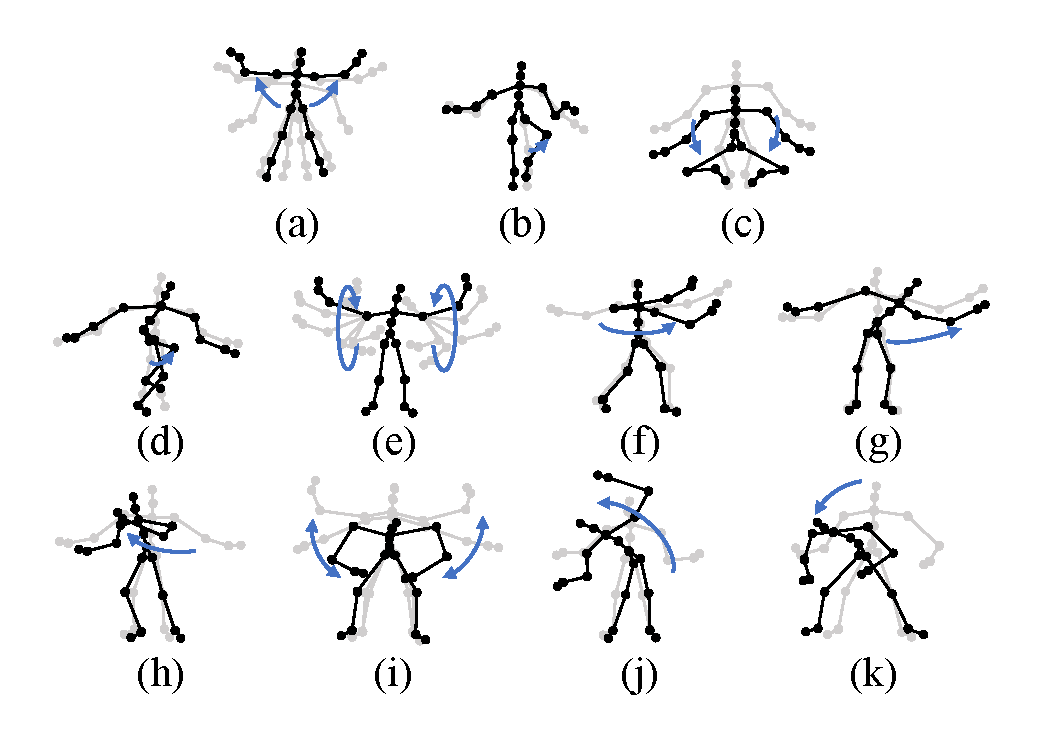
\includegraphics[scale=0.4]{fig/motion.pdf}
	\caption{Motions included in exercise motion: (a) jumping
jack, (b) jogging, (c) squatting, (d) knee raise, (e) arm circle, (f) twist, (g) side reach, (h) boxing, (i) arm wave, (j) side bend, and (k) toe touch.}
	\label{fig:motion}
	\vspace{-0.4cm}
\end{figure}
%
データは4 fpsにダウンサンプリングし,左手・右手・左足・右足の
2次元位置座標からなる8次元データを使用した.各座標はmin-max正規化により,値の範囲を[−1, 1]に正規化した.

本実験では,従来手法であるGP-HSMMに加え,ランダムフーリエ特徴(Random Fourier Features, RFF)を導入した
2種類のRFF-GP-HSMMモデルを用いて学習を行った.1つはMCMCを導入していないRFF-GP-HSMM,もう1つはカーネル近似の
精度向上のためにMCMCを導入したRFF-GP-HSMMである.いずれのRFF-GP-HSMMにおいても,ランダム特徴数は$M=20$に設定した.
すべての手法において,セグメント長パラメータは$\lambda=20$,最小セグメント長$K_{\min}=15$,
最大セグメント長$K_{\max}=30$とし,ブロック化ギブスサンプラーの繰り返し回数は5回とした.

2つ目の実験では,AAAI~2024にて提案されたDanceMVP\cite{DanceMVP2024}に基づく公式ダンスデータセット\footnote{https://github.com/YunZhongNikki/ImperialDance-Dataset}を用いた.
本データセットでは,TWICEの楽曲「What is Love?」の10秒間の振り付けを踊った動作
が記録されており,21個の関節に対する3次元($x, y, z$)座標からなる63次元の座標データを含む.本実験ではこの動作データを使用する.
対象関節は,右膝,右つま先,右太もも,左太もも,左足,右肩,左手,右手,左前腕,左肩,右足,首,左膝,胸,頭,左つま先,腹,右上腕,左上腕,腰,右前腕である.
すべての関節の座標値から胸の座標を減算し,胸を原点とする相対座標に変換した.この処理により,
63次元から胸を基準とした60次元の座標データに変換した.

上級者によるダンス動作データとして,100 fpsで記録された1回あたり1,200フレームのデータの20回分を
初期モデルデータセットとして学習させた.さらに,中級者による同様のデータの20回分を追加データセットとして,
初期学習で得られた事後分布を事前分布とみなして逐次学習を行った.本実験で用いた全データは,2名の被験者に対して,
各20試行,1試行あたり1,200フレーム,1フレームあたり60次元の座標データから構成されており,総計2,880,000点の時系列データ
となる.

この実験では,MCMCおよび逐次学習の両方を導入したRFF-GP-HSMMと,従来のGP-HSMMとの比較を行った.
RFF-GP-HSMMではランダム特徴数を$M=20$に設定し,両手法においてセグメント長パラメータは$\lambda=120$,
最小セグメント長$K_{\min}=100$,最大セグメント長$K_{\max}=140$とし,ブロック化ギブスサンプラーの繰り返し回数は3回とした.
両実験において使用したPCの仕様はTable~\ref{table:mac}に示す.

\begin{table}[t]
\caption{Computer used in the experiments.}
\label{table:mac}
 \centering
\begin{tabular}{cc}
    \hline
    CPU & Apple M4 \\
    Memory & 16GB \\
    \hline
\end{tabular}
\end{table}

\subsection{Experiment 1: Segmentation Accuracy on the Exercise Dataset}\label{ITH}
本実験では,従来手法であるGP-HSMMに加え,Random Fourier Features(RFF)を導入した
2種類のRFF-GP-HSMMモデルを用いて体操動作の分節化を行った.1つはMCMCを導入していないRFF-GP-HSMM,
もう1つはカーネル近似の精度向上を目的としてMCMCを導入したRFF-GP-HSMMである.

分節精度の評価には,セクション\ref{setup}で述べた3つの体操動作系列を10回繰り返すことで得られた合計30系列のデータセットを
用いた.すべての手法において初期値に対する感度が高いため,各手法について10回の試行を行い,それぞれの試行における
分節結果と正解ラベルとの正規化ハミング距離(Normalized Hamming Distance, NHD)を算出した.NHDは$[0,1]$の
範囲をとり,0に近いほど分節結果と正解ラベルの一致度が高いことを示す.

Table~\ref{tab:nhd_results}には,各手法において10回の試行から得られた分節系列と正解ラベルとのNHDの平均値および標準偏差を示す.
その結果,MCMCを導入していないRFF-GP-HSMMは,RFFによる近似の導入により高速化を実現しつつも,
GP-HSMMに比べてやや精度が劣る結果となった.一方,MCMCを導入したRFF-GP-HSMMではカーネル近似の精度が向上し,
NHDの平均および標準偏差が改善され,従来手法であるGP-HSMMと同程度の分節精度を達成した.

\begin{table}[t]
  \caption{Normalized Hamming Distance (Mean ± Standard Deviation) from 10 Trials for Each Method.}
  \label{tab:nhd_results}
  \centering
  \begin{tabular}{lc}
    \hline
    \textbf{Method} & \textbf{NHD (Mean ± SD)} \\
    \hline
    GP-HSMM & 0.384 ± 0.0589 \\
    RFF-GP-HSMM & 0.445 ± 0.0759 \\
    RFF-MCMC-GP-HSMM & 0.408 ± 0.0427 \\
    \hline
  \end{tabular}
\end{table}

\subsection{Experiment 2: Efficient Analysis and Comparative Evaluation on the Dance Dataset}
本実験では,288万点の時系列データを含む大規模なダンスデータセットを用いて,
提案手法と従来手法であるGP-HSMMの学習時間を比較した.
それぞれの手法について5回の試行を行い,各々の試行で学習時間を計測した.
その結果をTable~\ref{tab:training_time}に示す.

\begin{table}[t]
  \centering
  \caption{Comparison of Training Times}
  \label{tab:training_time}
  \begin{tabular}{ccc}
    \hline
    \textbf{Trial} & \textbf{GP-HSMM (s)} & \textbf{RFF-MCMC-GP-HSMM (s)} \\
    \hline
    1 & $2.94 \times 10^5$ & $1.96 \times 10^2$ \\
    2 & $3.35 \times 10^5$ & $1.99 \times 10^2$ \\
    3 & $3.06 \times 10^5$ & $1.98 \times 10^2$ \\
    4 & $3.02 \times 10^5$ & $1.90 \times 10^2$ \\
    5 & $3.28 \times 10^5$ & $1.95 \times 10^2$ \\
    \hline
    \textbf{Mean} & $\mathbf{3.13 \times 10^5}$ & $\mathbf{1.95 \times 10^2}$ \\
    \hline
  \end{tabular}
\end{table}


5回試行の平均値を比較すると,従来手法のGP-HSMMでは学習完了におよそ87時間を要したのに対し,
提案手法ではわずか約3分で学習が完了し,実用的な処理時間での解析が可能であることが確認された.

また本実験では,提案手法における逐次学習の枠組みに基づき,上級者のダンスデータを
初期モデルデータセット $\bX_c^{(1)}$ として用い,式(\ref{eq:rff_mu})に基づいて得られる
$\bS^{(1)}$,$\bm^{(1)}$ を初期の事後分布パラメータとした.その後,中級者のデータ $\bX_c^{(2)}$ を
追加データセットとして与え,式(\ref{eq:inc_S}),(\ref{eq:inc_m})に従って事後分布パラメータ $\bS^{(2)}$,$\bm^{(2)}$ を更新した.
このようにして得られた $\bm^{(1)}$,$\bm^{(2)}$ はそれぞれ,上級者および中級者の動作に基づく
関節の出力分布の平均ベクトルに対応しており,これらを用いることで各振り付け単位における熟練度の違いを関節ごとに定量的に可視化した.

提案手法により得られた分節結果に基づいて,ダンス動作は自動的に6種類の振り付けに分類された.
抽出された6つの振り付けの一例をFig.~\ref{fig:choreography}に示す.さらに,各振り付けに対して,
上級者および中級者の動作を比較するために,各関節ごとの60次元の $\bm^{(1)}$,$\bm^{(2)}$ を
主成分分析(PCA)により次元削減し,その結果を振り付けごとに可視化した.
%
\begin{figure}[t]
	\centering
	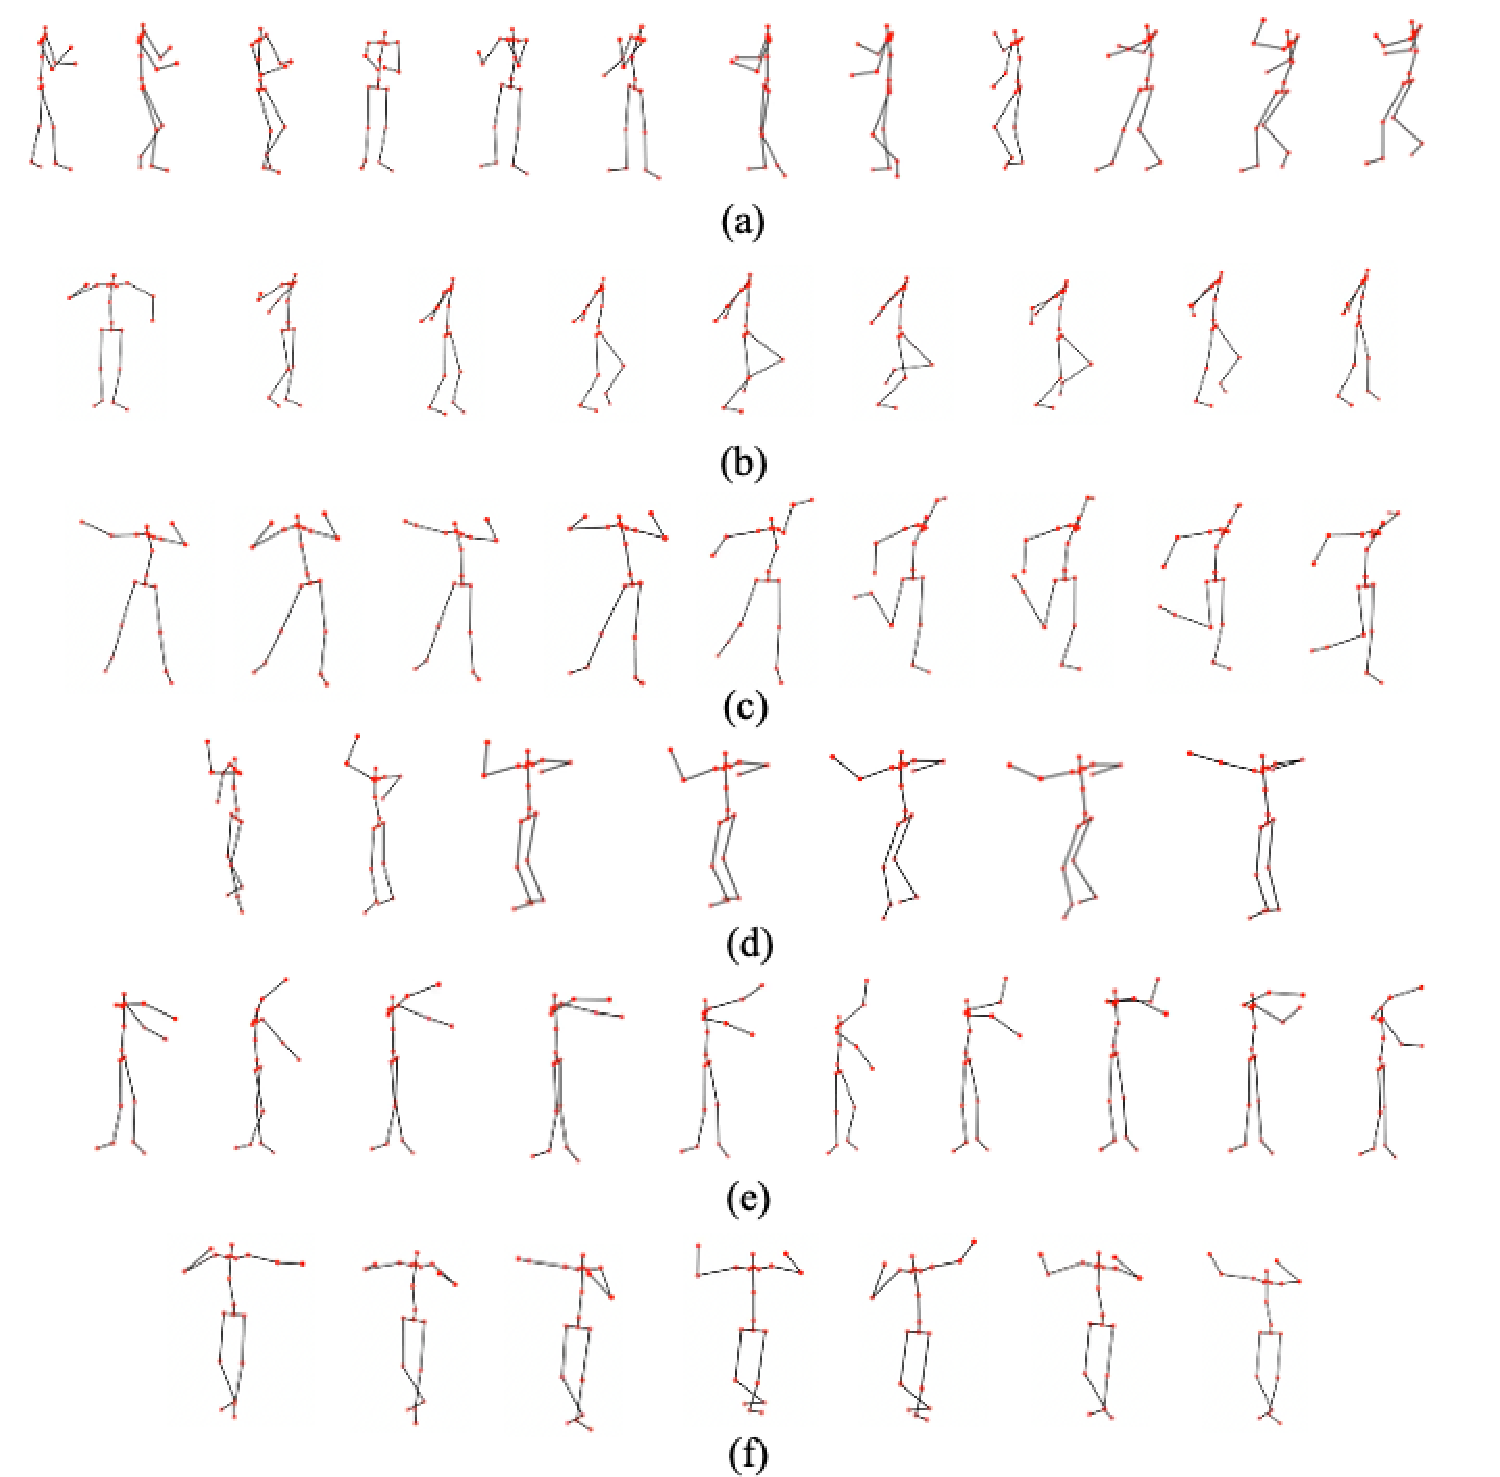
\includegraphics[scale=0.3]{fig/choreography.pdf}
	\caption{Choreographies: (a) Choreography 1: Swing both arms to the sides, 
  (b) Choreography 2: Raise and lower the left leg while bending the knee, 
  (c) Choreography 3: Swing the right arm back and forth while lifting the right heel, 
  (d) Choreography 4: Extend the left arm forward, 
  (e) Choreography 6: Swing the arm to the left side, 
  (f) Choreography 7: Stretch both arms to the sides.}
	\label{fig:choreography}
	\vspace{-0.4cm}
\end{figure}
%
分析結果として,Fig.~\ref{fig:choreography}に示す6つの振り付けについて,上級者の関節ごとの
事後分布の平均を青い丸印で示し,中級者のものをオレンジ色のバツ印で示した.特に動作の差異が顕著に現れた関節として,
左膝・左手・右前腕の3箇所に注目した.

%
\begin{figure}[t]
	\centering
	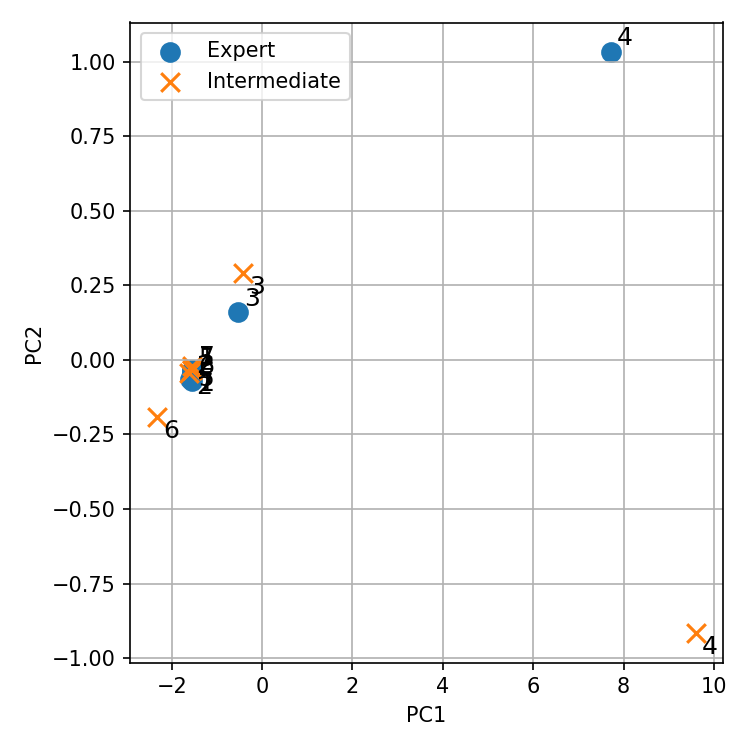
\includegraphics[scale=0.45]{fig/LShin.pdf}
	\caption{PCA result of the left knee}
	\label{fig:LShin}
	\vspace{-0.4cm}
\end{figure}
%

%
\begin{figure}[t]
	\centering
	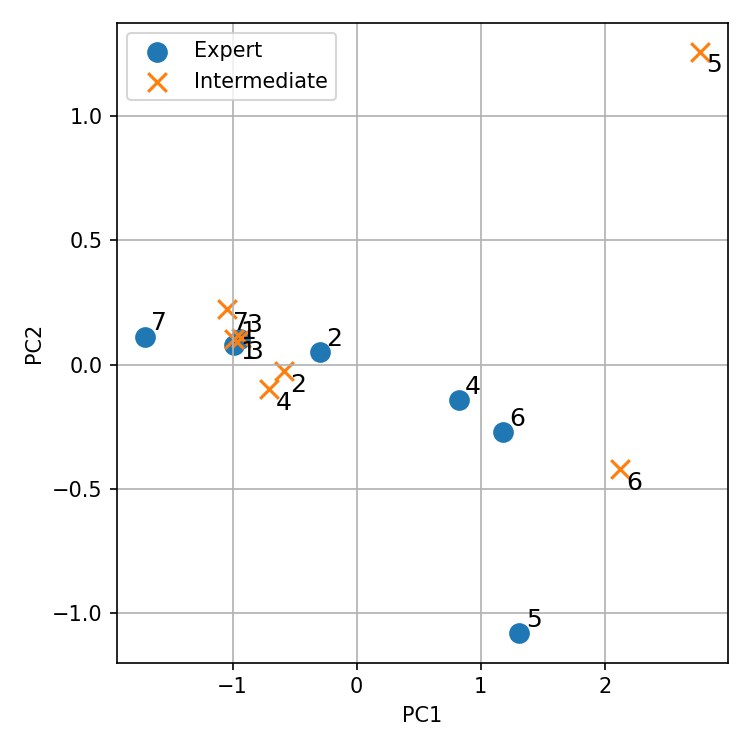
\includegraphics[scale=0.45]{fig/LHand.pdf}
	\caption{PCA result of the left hand}
	\label{fig:LHand}
	\vspace{-0.4cm}
\end{figure}
%

%
\begin{figure}[t]
	\centering
	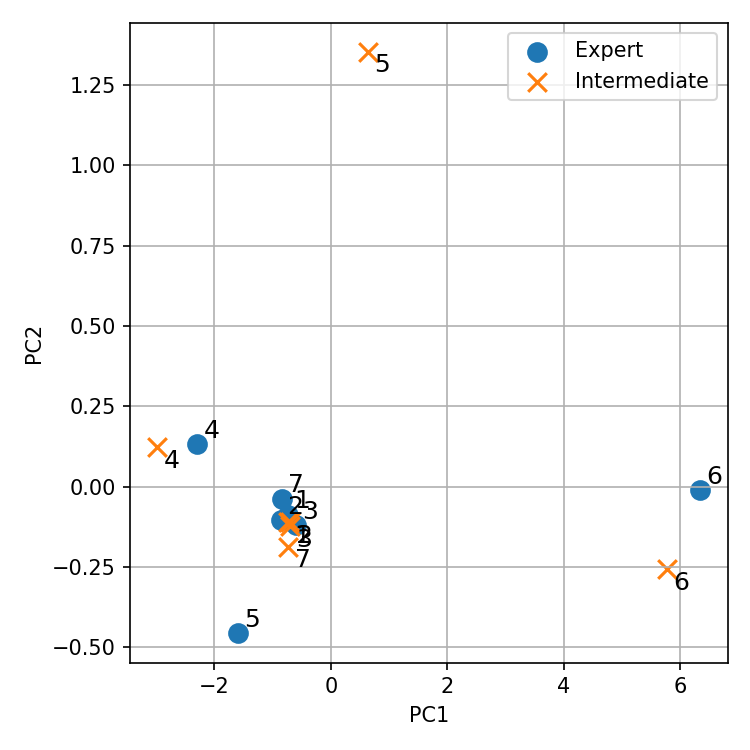
\includegraphics[scale=0.45]{fig/RFArm.pdf}
	\caption{PCA result of the right forearm}
	\label{fig:RFarm}
	\vspace{-0.4cm}
\end{figure}
%

%
\begin{figure}[t]
	\centering
	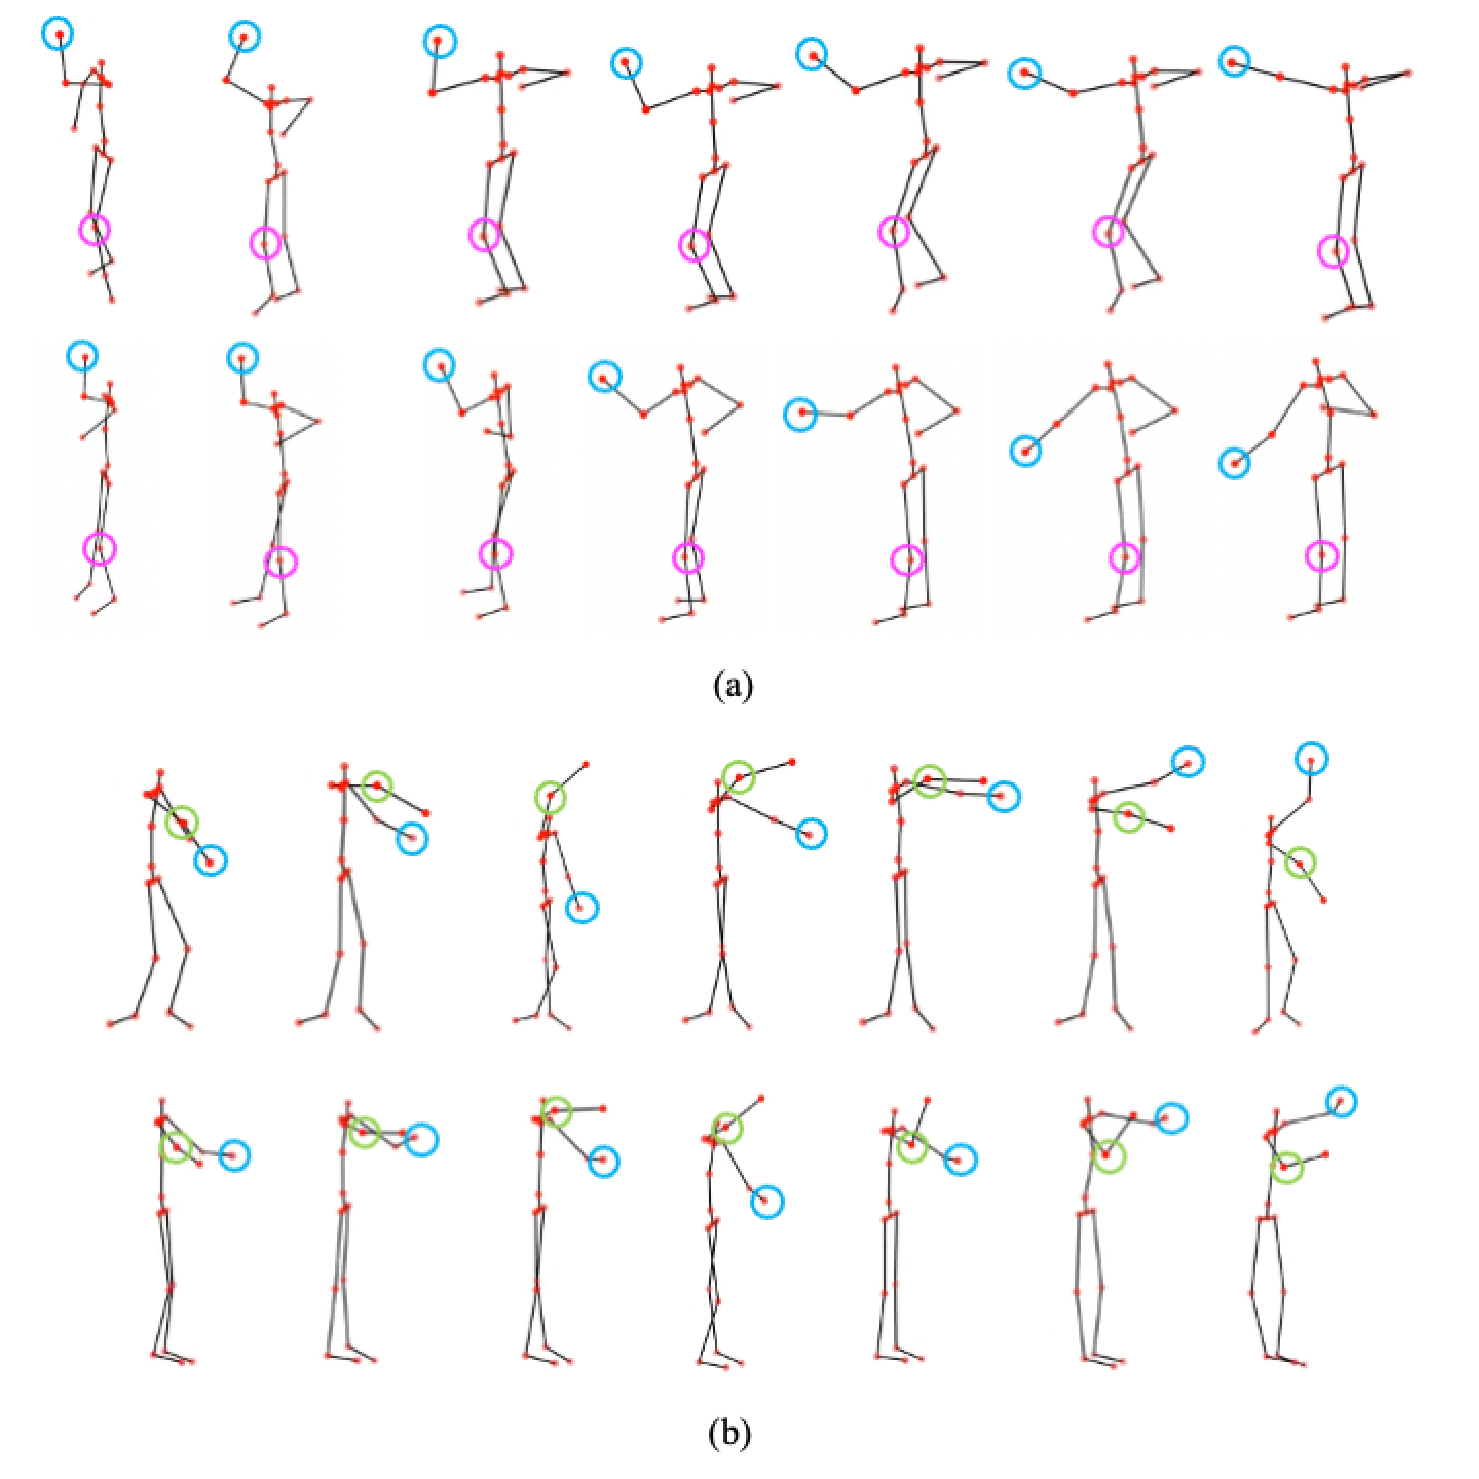
\includegraphics[scale=0.3]{fig/resultmotion.pdf}
	\caption{(a) Visualized movement of Choreography 4 segmented for detailed comparison.
  (b) Visualized movement of Choreography 5 segmented for detailed comparison.}
	\label{fig:resultmotion}
	\vspace{-0.4cm}
\end{figure}
%
まず,Fig.~\ref{fig:LShin} に示す左膝のPCA分析結果では,振り付け4において,
上級者と中級者の分布が乖離しており,特に膝を深く曲げる動作に対応する上級者の特徴が明確に現れていた.
次に,Fig.~\ref{fig:LHand} に示す左手のPCA分析結果では,振り付け4および5において,
上級者と中級者の分布に明確な差が見られ,両者の動作に違いがあることが示唆された.
最後に,Fig.~\ref{fig:RFarm} に示す右前腕のPCA分析結果では,振り付け5において,
上級者と中級者の分布に明瞭な差異が確認された.

これらのPCA分析結果で示された差異をより具体的に検証するため,分節化して
得られた振り付け4および5の動作をFig.~\ref{fig:resultmotion} (a),(b)にそれぞれ示す.
この図では,各振り付けにおいて上段が上級者,下段が中級者による動作を示し,時系列順にスライドとして並べている.
また,解析対象部位を強調するために,左手は水色の円,左膝はマゼンタ色の円,右前腕は黄緑色の円で囲って表示している.

Fig.~\ref{fig:resultmotion} (a)に示す振り付け4の動作スライドを用いて,各部位ごとに動作の違いを考察する.
まず,左膝に関しては,上級者がしっかりと膝を曲げているのに対し,中級者は膝の屈曲がほとんどないという様子が確認された.
次に,左手の動きに注目すると,上級者は左手を大きく前方に振り出すことで,動作にリズム感と力強さを与えているのに対し,中級者は手の前方への動きが不十分で,手が徐々に下がっていく傾向が見られた.

Fig.~\ref{fig:resultmotion} (b)に示す振り付け5の動作では,左手に関して,上級者は中級者よりも大きく振る動きを
行っており,PCA結果の差異と一致する傾向が確認できた.さらに,右前腕に関しても,上級者は右前腕を大きく使って
ダイナミックな動作をしているのに対し,中級者は右前腕の動きが小さく,動作が抑制されている様子が視覚的に確認できた.

これらの結果から,逐次学習を導入した提案手法により,熟練度の異なる複数の被験者の動作を振り付け単位で定量的かつ視覚的
に比較可能な支援システムを構築できることが示された.また,各振り付けにおいて,どの関節の動作を改善すれば上級者に
近づけるかを定量的に可視化・評価できることが明らかとなり,運動指導やフィードバックへの応用可能性が示唆された.

\section{Conclusion}
本研究では,ダンスやスポーツなど熟練度の異なる複数人の動作を振り付け単位で定量的かつ視覚的に比較可能な支援システムの開発
を目的とし,Gaussian Process Hidden Semi-Markov Model(GP-HSMM)を拡張した新たなフレームワークを提案した.提案手法では,
ガウス過程のカーネル近似にRandom Fourier Features(RFF)を用い,さらにマルコフ連鎖モンテカルロ法(MCMC)により
その近似精度を統計的に最適化することで,従来のGP-HSMMと同等の分節化精度を維持しながら,計算時間の大幅な短縮を実現した.
加えて,逐次学習を導入することで,初期モデルデータセットで学習した熟練者の知見を活かしつつ,新たな被験者の動作を段階的に取り込むことが可能となり,
個人ごとの動作特性を柔軟にモデル化できるようになった.

体操およびダンスの公開モーションキャプチャデータセットに基づく実験を通じて,MCMCによるカーネル近似の安定化と
逐次学習による適応的なモデル更新の有効性が示され,動作単位での関節ごとの違いを定量的に評価し,動作改善のための
具体的なフィードバックを提供可能な支援システムを実現した.

今後は,本システムをスポーツやリハビリなど動作の質や熟練度比較が求められる分野へ応用し,熟練者との比較に基づく個別支援を実現することで,
実社会の課題解決に貢献できる基盤技術として発展させていく.

\section*{Acknowledgment}
This research was supported by AMED under Grant Number JP24wm0625124.  
The authors acknowledge the use of the CMU Motion Capture Database and the ImperialDance dataset in this study.

\begin{thebibliography}{00}
\bibitem{Balazia2018} M. Balazia and P. Sojka, ``Walker-independent gait recognition with CNN,'' in \textit{2018 25th IEEE International Conference on Image Processing (ICIP)}, 2018, pp. 4163--4167.
\bibitem{3DPW2018} F. von Marcard, B. Rosenhahn, M. J. Black, and G. Pons-Moll, ``3D people in the wild: From videos to accurate 3D human pose and shape,'' in \textit{Proc. IEEE Conf. on Computer Vision and Pattern Recognition (CVPR)}, 2018, pp. 2670--2679.
\bibitem{Thoker2021} F. M. Thoker, H. Doughty, and C. G. M. Snoek, “Skeleton‑Contrastive 3D Action Representation Learning,” in \textit{Proc. 29th ACM International Conference on Multimedia (MM ’21)}, Oct. 20--24, 2021, Virtual Event, China, pp. 1655--1663.
\bibitem{Lam2023} W. T. Lam, Y. M. Tang, and K. N. K. Fong, “A systematic review of the applications of markerless motion capture technology for clinical measurement in rehabilitation,” \textit{Journal of NeuroEngineering and Rehabilitation}, vol. 20, no. 1, pp. 1--26, 2023.
\bibitem{Suo2024} X. Suo, W. Tang, and Z. Li, “Motion capture technology in sports scenarios: A survey,” \textit{Sensors}, vol. 24, no. 9, pp. 2947, 2024.
\bibitem{DanceMVP2024} X. Li, S. Wu, Z. Yang, and L. Yi, ``DanceMVP: Multi-task dance performance assessment via text prompting,'' in \textit{Proc. AAAI Conf. Artificial Intelligence}, vol. 38, no. 9, 2024, pp. 10270--10278.
\bibitem{Nakamura2017} T. Nakamura, T. Nagai, D. Mochihashi, I. Kobayashi, H. Asoh, and M. Kaneko, “Segmenting continuous motions with hidden semi-Markov models and Gaussian processes,” \textit{Frontiers in Neurorobotics}, vol. 11, p. 67, 2017.
\bibitem{Rahimi2007} A. Rahimi and B. Recht, “Random features for large-scale kernel machines,” in \textit{Advances in Neural Information Processing Systems}, J. Platt, D. Koller, Y. Singer, and S. Roweis, Eds., vol. 20. \textit{Curran Associates, Inc.}, 2007.
\bibitem{Hastings1970} W. K. Hastings, “Monte Carlo sampling methods using Markov chains and their applications,” \textit{Biometrika}, vol. 57, no. 1, pp. 97--109, 1970.
\bibitem{Broderick2013} T. Broderick, N. Boyd, A. Wibisono, A. C. Wilson, and M. I. Jordan, “Streaming variational Bayes,” \textit{arXiv preprint} arXiv:1307.6769, 2013.
\bibitem{Fox2011} E. B. Fox, E. B. Sudderth, M. I. Jordan, and A. S. Willsky, “Joint modeling of multiple related time series via the beta process,” \textit{arXiv preprint} arXiv:1112.1414, 2011.
\bibitem{Matsubara2014} Y. Matsubara, Y. Sakurai, and C. Faloutsos, “Autoplait: Automatic mining of co-evolving time sequences,” in \textit{Proceedings of the 2014 ACM SIGMOD International Conference on Management of Data}, 2014, pp. 193--204.
\bibitem{Sener2018} F. Sener and A. Yao, “Unsupervised learning and segmentation of complex activities from video,” in \textit{Proceedings of the IEEE Conference on Computer Vision and Pattern Recognition}, 2018, pp. 8368--8376.
\bibitem{Bojanowski2014} P. Bojanowski, R. Lajugie, F. Bach, I. Laptev, J. Ponce, C. Schmid, and J. Sivic, “Weakly supervised action labeling in videos under ordering constraints,” in \textit{Computer Vision - ECCV 2014: 13th European Conference, Zurich, Switzerland, September 6--12, 2014, Proceedings, Part V}, \textit{Springer}, 2014, pp. 628-643.
\bibitem{Huang2016} D.-A. Huang, L. Fei-Fei, and J. C. Niebles, “Connectionist temporal modeling for weakly supervised action labeling,” in \textit{Computer Vision - ECCV 2016: 14th European Conference, Amsterdam, The Netherlands, October 11--14, 2016, Proceedings, Part IV}, \textit{Springer}, 2016, pp. 137--153.
\bibitem{Richard2017} A. Richard, H. Kuehne, and J. Gall, “Weakly supervised action learning with RNN based fine-to-coarse modeling,” in \textit{Proceedings of the IEEE Conference on Computer Vision and Pattern Recognition}, 2017, pp. 754-763.
\bibitem{Mimura2024} K. Mimura, J. Matsumoto, D. Mochihashi, T. Nakamura, H. Nishijo, M. Higuchi, T. Hirabayashi, and T. Minamimoto, “Unsupervised decomposition of natural monkey behavior into a sequence of motion motifs,” \textit{Communications Biology}, vol. 7, no. 1, p. 1080, 2024.
\bibitem{Saito2023a} I. Saito, T. Nakamura, T. Hatta, W. Fujita, S. Watanabe, and S. Miwa, “Unsupervised work behavior analysis using hierarchical probabilistic segmentation,” in \textit{IECON 2023-49th Annual Conference of the IEEE Industrial Electronics Society}, 2023, pp. 1--6.
\bibitem{Mo2023} Y. Mo, H. Sasaki, T. Matsubara, and K. Yamazaki, “Multi-step motion learning by combining learning-from-demonstration and policy-search,” \textit{Advanced Robotics}, vol. 37, no. 9, pp. 560--575, 2023. [Online]. Available: https://doi.org/10.1080/01691864.2022.2163187
\bibitem{Zhang2023} M. M. Zhang, G. W. Gundersen, and B. E. Engelhardt, “Bayesian non-linear latent variable modeling via random Fourier features,” \textit{arXiv preprint} arXiv:2306.08352, 2023.
\bibitem{Li2024} Y. Li, Z. Lin, F. Yin, and M. M. Zhang, “Preventing model collapse in Gaussian process latent variable models,” \textit{arXiv preprint} arXiv:2404.01697, 2024.
\bibitem{Jung2020} Y. Jung and J. Park, “Scalable hybrid HMM with Gaussian process emission for sequential time-series data clustering,” \textit{arXiv preprint} arXiv:2001.01917, 2020.
\end{thebibliography}

\vspace{12pt}

\end{document}
